\chapter{Symbol table}\label{ch:symboltable}
The compiler uses a symbol table to keep track of information relating to scope rules and name bindings.
The symbol table is used to keep track of which variables are declared in the program. 
Every time a new variable is declared, it gets added to the symbol table. 
This can be used to quickly look up if a variable is declared or if it is used in other contexts. 
It can also be used to check if a variable with the same name already exists when a new variable is declared.

\section{The symbol table mechanism}
A symbol table mechanism must allow for adding information and searching through the symbol table as effectively as possible.
When choosing a symbol table mechanism it is necessary to consider whether ease of implementation or search performance is valued highest \cite{Dragon}.
\\\\
\textbf{Linear list}
\\
A linear list is the easiest to implement, but has poor performance when the the number of entries and the number of inquiries get large, since it will have to go through the entries linearly. 
This means it has a worst case complexity of $O(n)$ and an average case of $\Theta(n)$. 
\\\\
\textbf{Hash table}
\\
A hash table has better performance when dealing with a large number of entries and inquiries, but is harder to implement. Like the linear list mentioned above, it has a worst case complexity of $O(n)$, however the average case is $\Theta(1)$.
The hash table is a widely used mechanism for symbol table implementations \cite{CraftinfACompiler}.

\section{The symbol table entries}
Within the symbol table each entry is the declaration of a name. 
The format for entries does not have to be uniform since the information saved around a given name depends on the usage of the name. 
It might be an advantage, however, to keep it uniform since it can be more easily read.
\\\\
One way to accomplish this might be to store a pointer to the name, in a separate array, which has a fixed size as shown on figure~\ref{fig:FixedSize}, as opposed to making the field a fixed size where a large overhead can occur as shown on figure~\ref{fig:SeparateArray}.
\begin{figure}[H]
\centering
  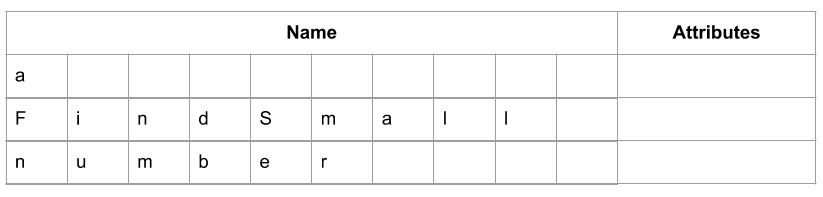
\includegraphics[width=\textwidth]{figures/FixedSize.png}
  \caption{This figure shows how the table can be formed using fixed sized field \cite{Dragon}}
  \label{fig:FixedSize}
\end{figure}
\begin{figure}[H]
\centering
  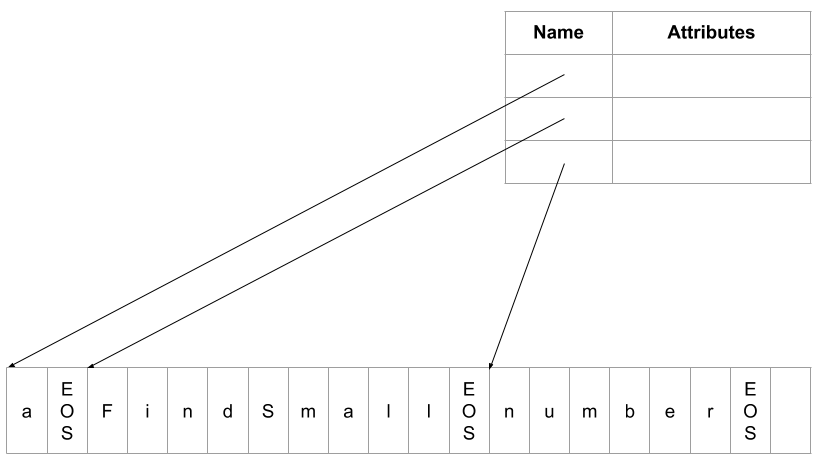
\includegraphics[width=\textwidth]{figures/InSeparateArray.png}
  \caption{This figure shows how the table can be formed using an separate array \cite{Dragon}}
  \label{fig:SeparateArray}
\end{figure}
\noindent
In PHAL the hash table approach was chosen, due to the better average case performance. This will be further elaborated upon in Chapter~\ref{ch:bindingvisitor}.